\documentclass{article}
\usepackage[right=2cm, left=2cm, top=2cm, bottom=2cm]{geometry}
\usepackage{pgfplots}

%%%%%%%%%%%%%%%%%%%%%%%%%%%%%%%%%%%%%%%%%%%
% The following allows combinations of single
% columns, multicolumn and figures.
\usepackage{caption}
\usepackage{multicol}
\newenvironment{Figure}
  {\par\medskip\noindent\minipage{\linewidth}}
  {\endminipage\par\medskip}
%%%%%%%%%%%%%%%%%%%%%%%%%%%%%%%%%%%%%%%%%%%

\title{Event driven simulation of a granular gas}
\author{Jonas Bueie}
\date{\today}

\begin{document}
\large
\maketitle

\noindent \hrulefill
\section*{Abstract}

This report summarizes a computational experiment where a two dimensional granular gas has been simulted in an event driven simulation.

\noindent \hrulefill

\begin{multicols}{2}
\section{Introduction}

A granular gas is a two dimensional model in which a gas is represented by circular particles of finite raadii and masses, that can collide elastically or inellastically.
In this report, some results from simulations of suh a gas are given.
The simulations show results that are in agreement with staatistical mechanics.

\section{Theory}

\section{Results}
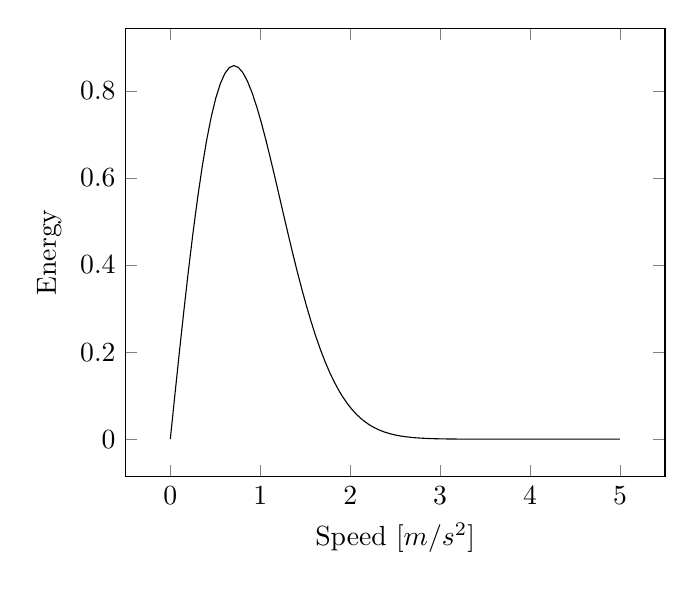
\begin{tikzpicture}
\begin{axis}[
    xlabel={Speed [$m/s^2$]},
    ylabel={Energy},
]
\addplot[
    domain=0:5,
    samples=100,
    color=black,
    ]
    {(2*x/1)*exp(-(x^2)/1)};
\end{axis}
\end{tikzpicture}


\begin{tikzpicture}
\begin{axis}[
    xlabel={Speed [$m/s^2$]},
    ylabel={Number of particles},
    xmin=0,
    ybar interval=0.5,
    bar width=2,
    enlargelimits=1,
]
\addplot table[
    y expr = \thisrow{v_0},
    ]{../data/task_1_speeds.csv};
;
\addlegendentry{Maxwell distribution}
\end{axis}
\end{tikzpicture}

\begin{tikzpicture}
\begin{axis}[
    xlabel={Speed [$m/s^2$]},
    ylabel={Number of particles},
    xmin=0,
    ybar interval=0.5,
    bar width=2,
    enlargelimits=1,
]
\addplot table[
    y expr = \thisrow{v_1},
    ]{../data/task_1_speeds.csv};
\addlegendentry{Maxwell distribution}
\end{axis}
\end{tikzpicture}

\begin{tikzpicture}
\begin{axis}[
    xlabel={Time},
    ylabel={Kinetic energy},
]
\addplot [
    mark=none,
    ]table{../data/task_30.8_energy.csv};
\addlegendentry{Maxwell distribution}
\end{axis}
\end{tikzpicture}

\end{multicols}
\end{document}

